% Created by tikzDevice version 0.12.6 on 2024-03-12 19:53:22
% !TEX encoding = UTF-8 Unicode
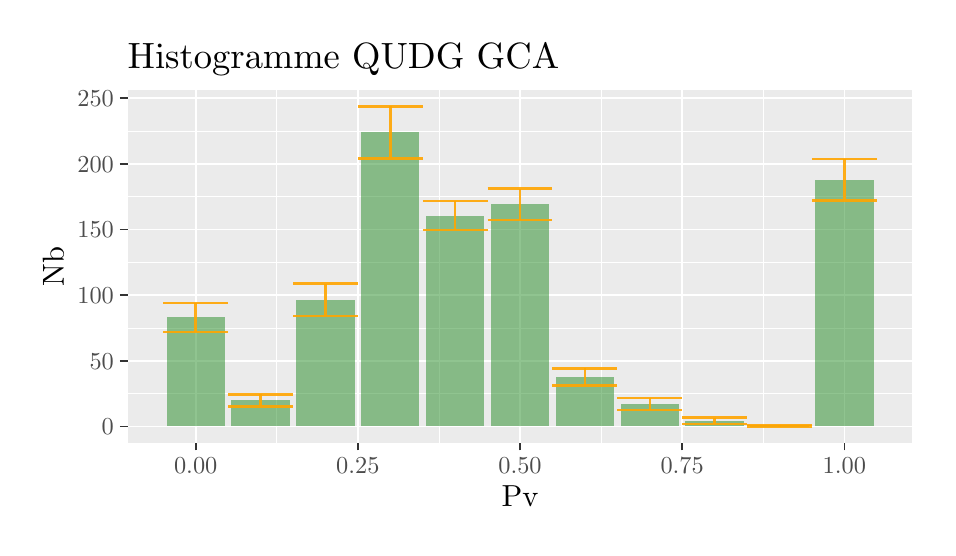
\begin{tikzpicture}[x=1pt,y=1pt]
\definecolor{fillColor}{RGB}{255,255,255}
\path[use as bounding box,fill=fillColor,fill opacity=0.00] (0,0) rectangle (325.21,180.67);
\begin{scope}
\path[clip] (  0.00,  0.00) rectangle (325.21,180.67);
\definecolor{drawColor}{RGB}{255,255,255}
\definecolor{fillColor}{RGB}{255,255,255}

\path[draw=drawColor,line width= 0.6pt,line join=round,line cap=round,fill=fillColor] (  0.00,  0.00) rectangle (325.21,180.68);
\end{scope}
\begin{scope}
\path[clip] ( 36.11, 30.69) rectangle (319.71,158.02);
\definecolor{fillColor}{gray}{0.92}

\path[fill=fillColor] ( 36.11, 30.69) rectangle (319.71,158.02);
\definecolor{drawColor}{RGB}{255,255,255}

\path[draw=drawColor,line width= 0.3pt,line join=round] ( 36.11, 48.45) --
	(319.71, 48.45);

\path[draw=drawColor,line width= 0.3pt,line join=round] ( 36.11, 72.17) --
	(319.71, 72.17);

\path[draw=drawColor,line width= 0.3pt,line join=round] ( 36.11, 95.90) --
	(319.71, 95.90);

\path[draw=drawColor,line width= 0.3pt,line join=round] ( 36.11,119.62) --
	(319.71,119.62);

\path[draw=drawColor,line width= 0.3pt,line join=round] ( 36.11,143.35) --
	(319.71,143.35);

\path[draw=drawColor,line width= 0.3pt,line join=round] ( 90.02, 30.69) --
	( 90.02,158.02);

\path[draw=drawColor,line width= 0.3pt,line join=round] (148.62, 30.69) --
	(148.62,158.02);

\path[draw=drawColor,line width= 0.3pt,line join=round] (207.21, 30.69) --
	(207.21,158.02);

\path[draw=drawColor,line width= 0.3pt,line join=round] (265.81, 30.69) --
	(265.81,158.02);

\path[draw=drawColor,line width= 0.6pt,line join=round] ( 36.11, 36.59) --
	(319.71, 36.59);

\path[draw=drawColor,line width= 0.6pt,line join=round] ( 36.11, 60.31) --
	(319.71, 60.31);

\path[draw=drawColor,line width= 0.6pt,line join=round] ( 36.11, 84.04) --
	(319.71, 84.04);

\path[draw=drawColor,line width= 0.6pt,line join=round] ( 36.11,107.76) --
	(319.71,107.76);

\path[draw=drawColor,line width= 0.6pt,line join=round] ( 36.11,131.49) --
	(319.71,131.49);

\path[draw=drawColor,line width= 0.6pt,line join=round] ( 36.11,155.21) --
	(319.71,155.21);

\path[draw=drawColor,line width= 0.6pt,line join=round] ( 60.72, 30.69) --
	( 60.72,158.02);

\path[draw=drawColor,line width= 0.6pt,line join=round] (119.32, 30.69) --
	(119.32,158.02);

\path[draw=drawColor,line width= 0.6pt,line join=round] (177.91, 30.69) --
	(177.91,158.02);

\path[draw=drawColor,line width= 0.6pt,line join=round] (236.51, 30.69) --
	(236.51,158.02);

\path[draw=drawColor,line width= 0.6pt,line join=round] (295.10, 30.69) --
	(295.10,158.02);
\definecolor{fillColor}{RGB}{34,139,34}

\path[fill=fillColor,fill opacity=0.50] ( 50.17, 36.59) rectangle ( 71.27, 76.00);

\path[fill=fillColor,fill opacity=0.50] ( 73.61, 36.59) rectangle ( 94.71, 45.99);

\path[fill=fillColor,fill opacity=0.50] ( 97.05, 36.59) rectangle (118.15, 82.31);

\path[fill=fillColor,fill opacity=0.50] (120.49, 36.59) rectangle (141.58,142.83);

\path[fill=fillColor,fill opacity=0.50] (143.93, 36.59) rectangle (165.02,112.77);

\path[fill=fillColor,fill opacity=0.50] (167.37, 36.59) rectangle (188.46,116.84);

\path[fill=fillColor,fill opacity=0.50] (190.80, 36.59) rectangle (211.90, 54.45);

\path[fill=fillColor,fill opacity=0.50] (214.24, 36.59) rectangle (235.34, 44.70);

\path[fill=fillColor,fill opacity=0.50] (237.68, 36.59) rectangle (258.78, 38.58);

\path[fill=fillColor,fill opacity=0.50] (261.12, 36.59) rectangle (282.21, 36.79);

\path[fill=fillColor,fill opacity=0.50] (284.56, 36.59) rectangle (305.65,125.69);
\definecolor{drawColor}{RGB}{255,165,0}

\path[draw=drawColor,draw opacity=0.90,line width= 0.9pt,line join=round] ( 49.00, 81.21) --
	( 72.44, 81.21);

\path[draw=drawColor,draw opacity=0.90,line width= 0.9pt,line join=round] ( 60.72, 81.21) --
	( 60.72, 70.78);

\path[draw=drawColor,draw opacity=0.90,line width= 0.9pt,line join=round] ( 49.00, 70.78) --
	( 72.44, 70.78);

\path[draw=drawColor,draw opacity=0.90,line width= 0.9pt,line join=round] ( 72.44, 48.18) --
	( 95.88, 48.18);

\path[draw=drawColor,draw opacity=0.90,line width= 0.9pt,line join=round] ( 84.16, 48.18) --
	( 84.16, 43.80);

\path[draw=drawColor,draw opacity=0.90,line width= 0.9pt,line join=round] ( 72.44, 43.80) --
	( 95.88, 43.80);

\path[draw=drawColor,draw opacity=0.90,line width= 0.9pt,line join=round] ( 95.88, 88.17) --
	(119.32, 88.17);

\path[draw=drawColor,draw opacity=0.90,line width= 0.9pt,line join=round] (107.60, 88.17) --
	(107.60, 76.44);

\path[draw=drawColor,draw opacity=0.90,line width= 0.9pt,line join=round] ( 95.88, 76.44) --
	(119.32, 76.44);

\path[draw=drawColor,draw opacity=0.90,line width= 0.9pt,line join=round] (119.32,152.23) --
	(142.76,152.23);

\path[draw=drawColor,draw opacity=0.90,line width= 0.9pt,line join=round] (131.04,152.23) --
	(131.04,133.44);

\path[draw=drawColor,draw opacity=0.90,line width= 0.9pt,line join=round] (119.32,133.44) --
	(142.76,133.44);

\path[draw=drawColor,draw opacity=0.90,line width= 0.9pt,line join=round] (142.76,118.02) --
	(166.19,118.02);

\path[draw=drawColor,draw opacity=0.90,line width= 0.9pt,line join=round] (154.47,118.02) --
	(154.47,107.52);

\path[draw=drawColor,draw opacity=0.90,line width= 0.9pt,line join=round] (142.76,107.52) --
	(166.19,107.52);

\path[draw=drawColor,draw opacity=0.90,line width= 0.9pt,line join=round] (166.19,122.50) --
	(189.63,122.50);

\path[draw=drawColor,draw opacity=0.90,line width= 0.9pt,line join=round] (177.91,122.50) --
	(177.91,111.19);

\path[draw=drawColor,draw opacity=0.90,line width= 0.9pt,line join=round] (166.19,111.19) --
	(189.63,111.19);

\path[draw=drawColor,draw opacity=0.90,line width= 0.9pt,line join=round] (189.63, 57.58) --
	(213.07, 57.58);

\path[draw=drawColor,draw opacity=0.90,line width= 0.9pt,line join=round] (201.35, 57.58) --
	(201.35, 51.32);

\path[draw=drawColor,draw opacity=0.90,line width= 0.9pt,line join=round] (189.63, 51.32) --
	(213.07, 51.32);

\path[draw=drawColor,draw opacity=0.90,line width= 0.9pt,line join=round] (213.07, 46.87) --
	(236.51, 46.87);

\path[draw=drawColor,draw opacity=0.90,line width= 0.9pt,line join=round] (224.79, 46.87) --
	(224.79, 42.54);

\path[draw=drawColor,draw opacity=0.90,line width= 0.9pt,line join=round] (213.07, 42.54) --
	(236.51, 42.54);

\path[draw=drawColor,draw opacity=0.90,line width= 0.9pt,line join=round] (236.51, 39.79) --
	(259.95, 39.79);

\path[draw=drawColor,draw opacity=0.90,line width= 0.9pt,line join=round] (248.23, 39.79) --
	(248.23, 37.37);

\path[draw=drawColor,draw opacity=0.90,line width= 0.9pt,line join=round] (236.51, 37.37) --
	(259.95, 37.37);

\path[draw=drawColor,draw opacity=0.90,line width= 0.9pt,line join=round] (259.95, 37.11) --
	(283.39, 37.11);

\path[draw=drawColor,draw opacity=0.90,line width= 0.9pt,line join=round] (271.67, 37.11) --
	(271.67, 36.47);

\path[draw=drawColor,draw opacity=0.90,line width= 0.9pt,line join=round] (259.95, 36.47) --
	(283.39, 36.47);

\path[draw=drawColor,draw opacity=0.90,line width= 0.9pt,line join=round] (283.39,133.13) --
	(306.82,133.13);

\path[draw=drawColor,draw opacity=0.90,line width= 0.9pt,line join=round] (295.10,133.13) --
	(295.10,118.24);

\path[draw=drawColor,draw opacity=0.90,line width= 0.9pt,line join=round] (283.39,118.24) --
	(306.82,118.24);
\end{scope}
\begin{scope}
\path[clip] (  0.00,  0.00) rectangle (325.21,180.67);
\definecolor{drawColor}{gray}{0.30}

\node[text=drawColor,anchor=base east,inner sep=0pt, outer sep=0pt, scale=  0.88] at ( 31.16, 33.55) {0};

\node[text=drawColor,anchor=base east,inner sep=0pt, outer sep=0pt, scale=  0.88] at ( 31.16, 57.28) {50};

\node[text=drawColor,anchor=base east,inner sep=0pt, outer sep=0pt, scale=  0.88] at ( 31.16, 81.01) {100};

\node[text=drawColor,anchor=base east,inner sep=0pt, outer sep=0pt, scale=  0.88] at ( 31.16,104.73) {150};

\node[text=drawColor,anchor=base east,inner sep=0pt, outer sep=0pt, scale=  0.88] at ( 31.16,128.46) {200};

\node[text=drawColor,anchor=base east,inner sep=0pt, outer sep=0pt, scale=  0.88] at ( 31.16,152.18) {250};
\end{scope}
\begin{scope}
\path[clip] (  0.00,  0.00) rectangle (325.21,180.67);
\definecolor{drawColor}{gray}{0.20}

\path[draw=drawColor,line width= 0.6pt,line join=round] ( 33.36, 36.59) --
	( 36.11, 36.59);

\path[draw=drawColor,line width= 0.6pt,line join=round] ( 33.36, 60.31) --
	( 36.11, 60.31);

\path[draw=drawColor,line width= 0.6pt,line join=round] ( 33.36, 84.04) --
	( 36.11, 84.04);

\path[draw=drawColor,line width= 0.6pt,line join=round] ( 33.36,107.76) --
	( 36.11,107.76);

\path[draw=drawColor,line width= 0.6pt,line join=round] ( 33.36,131.49) --
	( 36.11,131.49);

\path[draw=drawColor,line width= 0.6pt,line join=round] ( 33.36,155.21) --
	( 36.11,155.21);
\end{scope}
\begin{scope}
\path[clip] (  0.00,  0.00) rectangle (325.21,180.67);
\definecolor{drawColor}{gray}{0.20}

\path[draw=drawColor,line width= 0.6pt,line join=round] ( 60.72, 27.94) --
	( 60.72, 30.69);

\path[draw=drawColor,line width= 0.6pt,line join=round] (119.32, 27.94) --
	(119.32, 30.69);

\path[draw=drawColor,line width= 0.6pt,line join=round] (177.91, 27.94) --
	(177.91, 30.69);

\path[draw=drawColor,line width= 0.6pt,line join=round] (236.51, 27.94) --
	(236.51, 30.69);

\path[draw=drawColor,line width= 0.6pt,line join=round] (295.10, 27.94) --
	(295.10, 30.69);
\end{scope}
\begin{scope}
\path[clip] (  0.00,  0.00) rectangle (325.21,180.67);
\definecolor{drawColor}{gray}{0.30}

\node[text=drawColor,anchor=base,inner sep=0pt, outer sep=0pt, scale=  0.88] at ( 60.72, 19.68) {0.00};

\node[text=drawColor,anchor=base,inner sep=0pt, outer sep=0pt, scale=  0.88] at (119.32, 19.68) {0.25};

\node[text=drawColor,anchor=base,inner sep=0pt, outer sep=0pt, scale=  0.88] at (177.91, 19.68) {0.50};

\node[text=drawColor,anchor=base,inner sep=0pt, outer sep=0pt, scale=  0.88] at (236.51, 19.68) {0.75};

\node[text=drawColor,anchor=base,inner sep=0pt, outer sep=0pt, scale=  0.88] at (295.10, 19.68) {1.00};
\end{scope}
\begin{scope}
\path[clip] (  0.00,  0.00) rectangle (325.21,180.67);
\definecolor{drawColor}{RGB}{0,0,0}

\node[text=drawColor,anchor=base,inner sep=0pt, outer sep=0pt, scale=  1.10] at (177.91,  7.64) {Pv};
\end{scope}
\begin{scope}
\path[clip] (  0.00,  0.00) rectangle (325.21,180.67);
\definecolor{drawColor}{RGB}{0,0,0}

\node[text=drawColor,rotate= 90.00,anchor=base,inner sep=0pt, outer sep=0pt, scale=  1.10] at ( 13.08, 94.35) {Nb};
\end{scope}
\begin{scope}
\path[clip] (  0.00,  0.00) rectangle (325.21,180.67);
\definecolor{drawColor}{RGB}{0,0,0}

\node[text=drawColor,anchor=base west,inner sep=0pt, outer sep=0pt, scale=  1.32] at ( 36.11,166.08) {Histogramme QUDG GCA};
\end{scope}
\end{tikzpicture}
